In questo capitolo parler\`o dei dataset utilizzati e di come \`e stato impostato l'esperimento.

\section{Part-of-Speech (PoS) tagging}
In linguistica, il PoS tagging, \`e un processo che consisite nel raggruppare le parole di una frase in calssi dette, appunto, \emph{Part of Speech} o \emph{classi morfologiche}.
Questo raggruppamento, viene fatto sia in base alla definizione della parola stessa che al contesto in cui si trova.

Nella grammatica tradizionale, esistono un numero limitato di classi morfologiche (sostantivo, verbo, aggettivo, articolo, pronome, avverbo, congiunzione, preposizione, ecc..).

Ad esempio, possiamo classificare la frase \emph{Il cane abbaia.} in questo modo:

\centerline{Il\textbf{/ART} cane\textbf{/SOST} abbaia\textbf{/V} .\textbf{/PUNT}}

Tuttavia, chiaramente, esistono molte pi\`u classi di queste.
Per il pronome, possiamo trattare le forme singolari, plurali e possessive come classi distinte.
In molti linguaggi, inoltre, le parole possono essere distinte in base al loro ``caso'' o in base al genere.

Un esempio di classificazione pi\`u dettagliata pu\`o essere:

\begin{center}
Il\textbf{/ART:m:s}

cane\textbf{/SOST:m:s}

abbaia\textbf{/V:ind:pr:3:s}

.\textbf{/PUNT:sent}
\end{center}

In linguistica sono previste classi morfologiche per vari livelli di dettaglio, in base al modello di classificazione scelto.

Solitamente, in sistemi di PoS tagging computerizzati, vengono adottati modelli di classificazione che prevedono un numero elevato di classi (da 50 o pi\`u) e variano in base alla lingua adottata.
Esistono vari modelli comunemente accettati, quelli utilizzati per gli esperimenti di questa tesi sono:
\begin{itemize}
  \item Penn Treebank Tagset, composto da 42 classi e usato per la lingua inglese.
  \item Tanll Tagset, che conta fino a 328 classi ed \`e usato per la lingua italiana.
\end{itemize}

Esistono numerosi approcci al PoS-Tagging automatizzato.
Il seguente diagramma (Figura~\ref{fig:feedforwardNeuralNetwork}) cerca di raffigurare i vari metodi esistenti.
Tuttavia, la realt\`a \`e molto pi\`u complicata, in quanto molti sistemi di classificazione usano idee proprie di alcuni o tutti questi metodi.

\begin{figure}[tp]
  \centering
  \begin{center}
    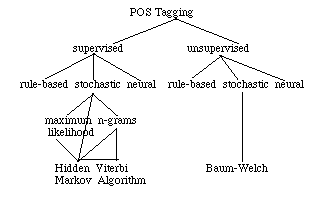
\includegraphics[width=0.7\textwidth]{./images/tagging_overview.png}
  \end{center}
  \caption{Metodi per il PoS-Tagging automatizzato.}
  \label{fig:feedforwardNeuralNetwork}
\end{figure}

\subsection{Supervisionato vs. non supervisionato}
\nocite{BrillMarcus:1993}
\nocite{Brill:1995}
\nocite{Shutze:1993}

Una delle prime distinzioni sugli algoritmi di PoS tagger esistanti pu\`o essere fatta in base al grado di automazione dei processi di addestramento e classificazione.
I termini comunemente utilizzati per questo tipo di distinzione sono \emph{supervisionato} e \emph{non supervisionato}.

I classificatori supervisionati sono tipicamente basati su corpus gi\`a taggati.
Questi fungono da base per creare qualsiasi strumento da usare durante tutto il processo di classificazione.
Ad esempio: il dizionario del classificatore, la frequenza parola/tag, la progabilit\`a di una sequanza di classi e/o l'insieme di regole per la classificazione.

I modelli non supervisionati, d'altro canto, non hanno bisogno di corpus taggati bens\`i usano sofisticati algoritmi di computazione per creare gruppi di parole (in altre parole, classi di parole), per poi utilizzare questi gruppi auto generati per calcolare le informazioni probabilistiche necessarie ad un classificatore stocastico oppure per generare le regole di contesto necessarie ad un classificatore basato su regole.

Il motivo principale per predilire un metodo completamente automatizzato (e quindi non supervisionato) al PoS tagging \`e che questo risulta essere estremamente portabile.
\`E risaputo, inoltre, che i classificatori automatici (supervisionati) tendono a performare meglio se addestrati e testati su una stessa tipologia di testi di quanto non possano fare i metodi completamente automatizzati.

Sfortunatamente, di corpus gi\`a taggati non ne esistono molti, soprattutto se si pensa alla moltitudine di lingue che possono richiedere una classificazione di questo tipo.
Anzi, il desiderio di automatizzare questo processo nasce proprio dalla necessit\`a di classificare con precisione testi che non sono stati classificati, in virt\`u del fatto che questo processo, se fatto manualmente, comporta un grande dispendio di tempo e risorse.

Tuttavia, l'approccio completamente automatizzato al PoS tagging porta con se altri incovenienti.
In particolare, i gruppi generati automaticamente da questi algoritmi, tendono ad essere molto grossolani e spessi si perde quella distinzione granulare che si trova in quei tag set appositamente studiati per un determinato linguaggio e utilizzati nei metodi supervisionati.

\subsection{Tagging basato su regole}
\nocite{Brill:1992}
\nocite{Greene:1971}

Di solito, gli approcci basati su regole usano informazioni di contesto per assegnare una classe a parole sconosciute o ambigue.
Queste regole, di solito, sono conosciute come regole \emph{context frame}.

Ad esempio, una regola di questo tipo pu\`o essere qualcosa del genere: se una parola $X$ ambigua/sconosciuta \`e preceduta da un \emph{determinante} ed e seguita da un \emph{nome}, allora $X$ \`e un aggettivo.

In aggiunta a queste informazioni di contesto, molti classificatori utilizzano informazioni di natura morfologica come aiuti nel processi di disambiguazione.
Una di queste regole potrebbe essere: se la parola ambigua/sconosciuta termina con il suffisso \emph{-ing} ed \`e preceduta da un verbo, allora eticettala come verbo (questo ovviamente \`e valido solo per l'inglese)

Alcuni sistemi si spingo anche oltre l'uso di informazioni morfologiche e contestuali, includendo regole che tengono conto anche della punteggiatura e della capitalizzazione.
Informazioni di questo tipo possono essere di grande o poca utilit\`a, in base al linguaggio il cui testo dev'essere classificato.
Per il tedesco, ad esempio, le informazioni riguardo la capitalizzazione delle lettere si \`e dimostrata essere estremamente utile nella classificazione di nomi sconosciuti.

I classificatori basati su regole molto spesso richiedono un addestramento di tipo supervisionato.
Tuttavia, recentemente, \`e aumentato l'interesse nei confronti dell'induzione automatica di regole.

Un approcco alla induzione automatica di regole consiste nel far classificare, ad un classificatore, del testo non classificato.
Un essere umano, poi, analizza il risultato della classificazione e corregge ogni parola erroneamente classificata.
Il testo, correttamente classificato, viene poi dato nuovamente in input al classificatore, che impara le regole di correzione confrontando i due insiemi di dati.

A volte \`e necessario ripetere questo processo pi\`u volte.

\subsection{Taggin stocastico}

Il termine ``tagger stocastico'' pu\`o essere utilizzato per indicare una grande variet\`a di approcci al problema del PoS tagging.
Infatti, ogni modello che, in qualche modo, utilizza il concetto di probabilit\`a o frequenza pu\`o essere etichettato correttamente come stocastico.

Il classificatore stocastico pi\`u semplice, disambigua le parole solamente in base alla probabilit\`a che una determinata parola occora con un particolare tag.
Quindi, per una determinata parola, il tag incontrato pi\`u di frequente nel training set, sar\`a anche quello assegnato a quella parola nel caso in cui la sua classificazione in un determinato contesto fosse ambigua.

Il problema con questo approccio \`e che, nonostante possa di certo restituire un tag valido per una data parola, pu\`o anche restituire una sequenza di tag del tutto non corretta.

Un'alternativa all'approccio basato sulla frequnza delle coppie parola/tag consiste nel calcolare la probabilit\`a dell'occorrenza di una data sequenza di tag.
Di solito, ci si riferisce a questo approccio con il termine \emph{n-gram}, il nome \`e dovuto al fatto che il tag migliore per una data parola viene determinato dalla probabilit\`a condizionata che questo occora dati gli \emph{n} tag precedenti.

L'algoritmo pi\`u comune per implementare l'approccio n-gram \`e conosciuto come \emph{Algoritmo Viterbi}.
Si tratta di un algoritmo di ricerca che evita l'espansione polinomiale di una ricerca per ampiezza ``potando'' l'albero di ricerca ad ogni livello usando le migliori $n$ \emph{Stime di Massima Verosomiglianza} (dove $n$ rappresenta il numero di possibili tag della parola seguente).

Il livello di complessit\`a successivo che pu\`o essere introdotto in un classificatore stocastico combina entrambi gli approcci precedenti, usando sia la probabilit\`a di una sequnza di tag che le misure della frequenza delle parole.
Questo approccio \`e conosciuto come \emph{Hidden Markov Model}.
Ogni stato nascosto di un tag produce una parola nella frase.

Le assunzioni alla base di questo modello sono le seguenti.

\begin{itemize}
  \item Ogni parola non \`e correlata con nessuna delle altre parole della frase e i rispettivi tag
  \item La probabilit\`a che una parola sia taggata in un determinato modo dipende dagli $n$ tag precedenti.
\end{itemize}

\subsection{Parole sconosciute}

Un problema rimane ancora in sospeso in relazione agli approcci descritti fino ad ora: come ci si dovrebbe comportare con le parole sconosciute?
Alcune delle regole di un classificatore basato su regole sono in grado di gestire questo problema, ma cosa accade in un modello stocastico?
Come \`e possibiel calcolare la probabilita che una data parola occorra con un dato tag, se quella parola e sconosciuta al classificatore?

Ci sono diversi possibili soluzioni a questo problema.
Uno consiste nell'usare informazioni di tipo morfologico.
In questo caso il classificatore calcola le probabilit\`a che un determinato suffisso, appartenente ad una parola sconosciuta, possa presentarsi con un particolare tag.

Un'altra soluzione consiste nell'assegnare, alla parola sconosciuta, un insieme di tag predefiniti (di solito si usa Nome, Verbo, Aggettivo e Avverbio), poi si cerca di disambiguare la parola usando la probabilit\`a che tale classe occorra dell'n-gram preso in considerazione.

Ancora, un'altra possibilit\`a \`e quella di calcolare la probabilit\`a che ogni tag del tag set ha di presentarsi alla fine dell'n-gram di riferimento, e di selezionare la calsse con la probabilit\`a pi\`a alta.
Tuttavia questa non \`e la soluzione ottimale, soprattutto quandi si utilizza un tag set molto grande.

\subsection{Preprocessing del testo}

\subsubsection{Tokenizzazione}
Il flusso di caratteri di un testo scritto in linguaggio naturale dev'essere necessariamente diviso in unit\`a di testo distinte e significative (detti token) prima che un qualsiasi tipo di processamento del linguaggio, che vada oltre il livello del carattere, possa essere eseguito.
Questo processo prende il nome di \emph{tokenizzazione}

Se un linguaggio \`e perfettamente punteggiato, la tokenizzazione \`e una cosa semplice da fare: un programma potrebbe estrarre parole e punteggiatura dal testo semplicemente dividendolo ad ogni spazio bianco e segno ti punteggiatura.

Ma nessun linguaggio reale \`e perfettamente punteggiato, e la situazione \`e sempre pi\`u complicata do cos\`i.
Anche in linguaggi ben (ma non perfettamente) punteggiato, come l'inglese, ci sono casi in cui la corretta tokenizzazione non pu\`o essere determinata semplicemente conoscendo la classificazione individuale di ciascun singolo carattere oltre a casi in cui sono possibili pi\`u tokenizzazioni per una stessa porzione di testo.

Ad esempio consideriamo la stringa, in inglese, ``\emph{chap.}'' .
Questa pu\`o essere interpretata sia come l'abbreviazione della parola \emph{chapter} che come la parola \emph{chap} alla fine di una frase.
Stessa cosa per la stringa ``\emph{Jan.}'', pu\`o essere interpretata sia come abbreviazione di \emph{January} che come il nome proprio \emph{Jan} alla fine di una frase.

Nel primo caso, il punto dev'essere considerato come parte del token mentre nel secondo caso dovrebbe essere considerato come un token a parte.

Nonostante lo spazio sia un indicatore abbastanza affidabile per individuare i confini dei token, ci sono parole, in inglese, che sono composte da pi\`u termini separate da uno spazio (ad esempio \emph{to and for}, \emph{jack rabbit}, \emph{General Motors}, \emph{a priori}).

Tutte queste difficolt\`a incontrate in un linguaggio come l'inglese sono relativamente limitate e alcune applicazioni di text-processing semplicemente le ignorano o le affrontano con algoritmi fatti ad hoc.

Ma tutte queste considerazioni sono state fatte su un solo linguaggio, altri linguaggi presentano problemi simili.
L'italiano, ad esempio, usa l'\emph{elisione} per gli articoli \emph{lo} e \emph{la}, quando questi incontrino una parola iniziante per vocale.
Il tedesco scrive i \emph{nomi composti}, ossia nomi formati dall'unione di pi\`u parole, senza spazi: \emph{Computerlinguistik} (linguistica computazionale).

Altri linguaggi offrono sfide ben pi\`u serie.
Il cinese, ad esempio, risulta essere scarsamente punteggiato e la forma pi\`u comune di cinese continentale non ha spazi bianchi e non \`e segmentato in alcun modo (come il greco che sulla stele di Rosetta).
Inoltre nel cinese la segmentazione \`e ambigua: due caratteri possono essere trattati come distinti ed avere un significato, oppure come un unico token ed averne un altro.

\`E evidente come il problema della tokenizzazione sia un problema fortemente dipendente dal linguaggio e va risolto caso per caso.

\section{Algoritmo utilizzato}

Tutti i PoS tagger esistenti, considerano la parola, o pi\`u generalmente il \emph{token}, come l'unit\`a fondamentale dell'apprendimento.
Molti algoritmi prevedono delle fasi di preprocessing del testo atte a semplificarlo, eliminando molte delle varianti tipiche di una lingua naturale, come ad esempio la \emph{lemmatizzazione}.

La lemmatizzazione consiste nel ridurre una forma \emph{flessa}\footnote{In linguistica si chiama \emph{flessione} una qualsiasi variazione morfologica delle parole realizzata per indicarne i tratti grammaticali o sintattici. Avremo ad esempio diverse forme flesse di un verbo (\emph{io lavoro}, \emph{tu lavori}) oppure di un nome (\emph{il lavoro}, \emph{i lavori}).} di una parola alla sua forma canonica (non marcata), detta \emph{lemma}\footnote{In linguistica si dice lemma la citazione di una parola, ossia quella parola che per convenzione è scelta per rappresentare tutte le forme di una flessione.}.
Esistono numerosi algoritmi di lemmatizzazione come, ad esempio, \emph{Lovins} e \emph{Porter}.
Entrambi sono algoritmi di \emph{suffix stripping} che rimuovono, quindi, i suffissi alle parole a partire da un dizionario di suffissi comuni.

Altro problema \`e la tokenizzazione, ossia la suddivisione del testo in token. Processo che all'apparenza sembra di semplice soluzione ma che nasconde delle difficolt\`a.
Prendiamo in considerazione \texttt{aren't}, qual \`e la tokenizzazione corretta? Possiamo infatti avvere \texttt{aren't}, \texttt{arent}, \texttt{are nt} e \texttt{aren t}.

I dizionari poi, vengono costruiti a partire alle parole presenti nel corpus.
La fase di preprocessing \`e fondamentale nella costruzione di un dizionario efficiente, altrimenti si avrebbero dizionari enormi con un elevto numero di parole che, pur avendo quasi lo stesso significato (es. \emph{lavoro}, \emph{lavori}) sono rappresentatio in maniera del tutto differente e senza alcuna correlazione.

In questa tesi si cercher\`a di cambiare approccio. L'unit\`a base sar\`a il singolo carattere, piuttosto che il token.
Questo approccio semplifica di molto la fase di preprocessing del testo, eliminandola del tutto.
Non sar\`a pi\`u necessario ne tokenizzare ne lemmatizzare il corpus in input.

Tuttavia sorgono alcuni problemi. La totalit\`a dei corpus taggati nonch\`e dei tagset esistenti, prevedono dei tag per le parole e non per i caratteri.
Quindi, per poter addestrare con successo la rete LSTM, risulta comunque necessario effettuare un minimo di preprocessing sui soli dataset utilizzati per l'addestramento.

Il preprocessing adottato consiste nel dividere le singole parole in singoli caratteri.
Ad ogni carattere \`e stato poi assegnato un tag che corrisponde al tag della parola dalla quale \`e stato estratto pi\`u un suffisso che ne indica la posizione nella parola:

\begin{itemize}
  \item il suffisso \emph{-S} (\emph{S}tart) per indicare il primo carattere di una parola
  \item il suffissio \emph{-I} (\emph{I}nner) per gli altri caratteri della parola
\end{itemize}

Ad esempio la

\begin{center}
  \begin{minipage}{5cm}
    \begin{verbatim}
     .
     reckons   VBZ
     .
     .
    \end{verbatim}
  \end{minipage}
\end{center}

diventa

\begin{center}
  \begin{minipage}{5cm}
    \begin{verbatim}
     .
     r   VBZ-S
     e   VBZ-I
     c   VBZ-I
     k   VBZ-I
     o   VBZ-I
     n   VBZ-I
     s   VBZ-I
     .
     .
    \end{verbatim}
  \end{minipage}
\end{center}

Un altro possibile problema riguarda la separazione fra le parole.
Nel PoS-Tagging tradizionale la separazione fra le parole \`e implicita, ogni token corrisponde ad una parola.
Nel nostro caso, non essendoci alcun tipo di tokenizzazione, si rischia di perdere un'informazione importante, ossia dove termina una parola e inizia un'altra.
Una soluzione consiste nell'aggiungere un carattere di spazio fra i caratteri delle singole parole ed assegnare a questo carattere il tag speciale \emph{S}.
Inoltre, non \`e che questa sia strettamente necessaria, la rete, infatti, potrebbe apprendere lo stesso questa informazione, grazie al suffissio dato ai tag (-S indica implicitamente l'inizio di una parola).
Difficile determinare a priori quale sia la scelta migliore, pertanto si \`e optato per adottarle entrambe addestrando pi\`u reti, met\`a delle quali con la soluzione dell'aggiungere il carattere di spazio e l'altra met\`a senza.

Dopo aver preprocessato i dataset, si passa alla creazione del dizionario.
Per ogni dataset sono stati creati 2 dizionari, uno contenente i soli tag, l'altro contenente tutti i caratteri dell'intero corpus.

Dal training set \`e stato estratto un piccolo insieme (~10\%) da usare come validation set.
La restante parte del training set \`e stato dato in input alla rete un carattere alla volta utilizzando la codifica \emph{one-hot}.

Questa consiste nel rappresentare una determinata informazione, nel nostro caso un carattere, mediante una sequenza di bit tutti posti a zero tranne uno.
In particolare, ipotizzando di avere un dizionario composto da $n$ caratteri, ciascun carattere sar\`a rappresentato mediante una sequenza di $n$ bit in questo modo:

\begin{itemize}
  \item il primo carattere sar\`a codificato con $1000000\dots0_{n}$
  \item il secondo carattere sar\`a codificato con $0100000\dots0_{n}$
  \item il terzo carattere sar\`a codificato con $0010000\dots0_{n}$
  \item e cos\`i via...
\end{itemize}

Il validation set \`e stato usato durante tutta la fase di addestramento per monitorarne l'andamento, calcolando periodicamente, su questo insieme di dati, il \emph{loss} (il valore dell'errore calcolato dalla funzione di perdita).

Per ogni dataset sono state addestrate 96 reti LSTM, ciascuna delle quali differisce dalle altre per:

\begin{itemize}
  \item numero di livelli (2, 3, 4, 5)
  \item numero di nodi (128, 256, 512, 1024)
  \item numero di fasi temporali (60, 80, 100)
  \item uso o meno del carattere di spazio
\end{itemize}

Ogni rete neurale \`e stata interrotta alla 150\textsuperscript{$\circ$} epoca.
Un'epoca corrisponde ad un passaggio completo dell'intero dataset attraverso la rete neurale.

Per valutare le prestazioni di ciascuna rete, sono stati usati i pesi corrispondenti all'epoca con il loss pi\`u basso.
A queste reti \`e stato poi dato in input il test set, un carattere alla volta, utilizzando lo stesso dizionario calcolato durante la fase di addestramento e con codifica one-hot.

La rete ha quindi classificato singolarmente tutti i caratteri del test set, dando a quest'utlimi una classe col suffisso \emph{-S} e \emph{-I}.
Da questa classificazione \`e stata poi estratta la classe della parola di appartenenza di ogni carattere scegliendola fra la classe di maggioranza dei singoli caratteri

Ad esempio, i caratteri della parola \texttt{reckons} sono stati classificati dalla rete neurale in questo modo:

\begin{center}
  \begin{minipage}{5cm}
    \begin{verbatim}
     .
     r   VBZ-S
     e   PRP-I
     c   VBZ-I
     k   VBZ-I
     o   NN-I
     n   VBZ-I
     s   VBD-I
     .
     .
    \end{verbatim}
  \end{minipage}
\end{center}

La classe che si ripete con pi\`u frequenza in questa sequenza di caratteri, a meno del suffisso, \`e \texttt{VBZ}, di conseguenza l'intera parola \texttt{reckons} \`e stata classificata come

\begin{center}
  \begin{minipage}{5cm}
    \begin{verbatim}
     reckons   VBZ
    \end{verbatim}
  \end{minipage}
\end{center}

\section{Dataset utilizzati}
\nocite{Zanchetta:2005}
\nocite{Attardi:2008}

\subsection{CoNLL 2000}
CoNLL (\emph{Conference on Natural Language Learning}), \`e una conferenza organizzata annualmente dal gruppo \emph{SIGNLL}, a partire dal 1999.
Per ogni edizione della conferenza, sono state proposte delle attivit\`a condivise, ciascuna delle quali comprendeva dati di test e di training forniti direttamente dagli organizzatori.
In questo modo i partecipanti potevano essere valutati e confrontati in maniera sistematica.

Per gli esperimenti di questa tesi, sono stati usati i dataset di training e test forniti durante la quarta edizione della conferenza, tenutasi nel 2000.
I dati forniti consistono in file di testo contenenti, complessivamente, $253\,906$ parole che formano $10\,729$ frasi, ogni riga di ciascun file di testo corrisponde ad una parola, mentre una riga vuota denota la fine di una frase.
Ciascuna riga \`e costituita, a sua volta, da 3 colonne:
\begin{itemize}
  \item la prima colonna contiene la parola corrente
  \item la seconda colonna la classe morfologica della parola
  \item la terza riga contiene un tag che indica la parte della frase a cui, la parola corrente, appartiene
\end{itemize}

Di seguito un esempio:

\begin{center}
  \begin{minipage}{5cm}
    \begin{verbatim}
     He        PRP  B-NP
     reckons   VBZ  B-VP
     the       DT   B-NP
     current   JJ   I-NP
     account   NN   I-NP
     deficit   NN   I-NP
     will      MD   B-VP
     narrow    VB   I-VP
     to        TO   B-PP
     only      RB   B-NP
     #         #    I-NP
     1.8       CD   I-NP
     billion   CD   I-NP
     in        IN   B-PP
     September NNP  B-NP
     .         .    O
    \end{verbatim}
  \end{minipage}
\end{center}

Di seguito la lista completa di classi del modello PennTreebank (Tabell~\ref{tab:penn-tagset}):

\begin{longtable}{| c | p{.40\textwidth} | p{.50\textwidth} |} \hline
  \thead{Tag} & \thead{Descrizione} & \thead{Esempio} \\ \hline
  CC & conjunction, coordinating & and, or, but \\ \hline
  CD & cardinal number & five, three, 13\% \\ \hline
  DT & determiner & the, a, these  \\ \hline
  EX & existential there & there were six boys  \\ \hline
  FW & foreign word & mais  \\ \hline
  IN & conjunction, subordinating or preposition & of, on, before, unless  \\ \hline
  JJ & adjective & nice, easy \\ \hline
  JJR & adjective, comparative & nicer, easier \\ \hline
  JJS & adjective, superlative & nicest, easiest  \\ \hline
  LS & list item marker &   \\ \hline
  MD & verb, modal auxillary & may, should  \\ \hline
  NN & noun, singular or mass & tiger, chair, laughter  \\ \hline
  NNS & noun, plural & tigers, chairs, insects  \\ \hline
  NNP & noun, proper singular & Germany, God, Alice  \\ \hline
  NNPS & noun, proper plural & we met two Christmases ago  \\ \hline
  PDT & predeterminer & both his children  \\ \hline
  POS & possessive ending & 's \\ \hline
  PRP & pronoun, personal & me, you, it  \\ \hline
  PRP\$ & pronoun, possessive & my, your, our  \\ \hline
  RB & adverb & extremely, loudly, hard   \\ \hline
  RBR & adverb, comparative & better  \\ \hline
  RBS & adverb, superlative & best  \\ \hline
  RP & adverb, particle & about, off, up  \\ \hline
  SYM & symbol & \%  \\ \hline
  TO & infinitival to & what to do?  \\ \hline
  UH & interjection & oh, oops, gosh  \\ \hline
  VB & verb, base form & think  \\ \hline
  VBZ & verb, 3rd person singular present & she thinks  \\ \hline
  VBP & verb, non-3rd person singular present & I think  \\ \hline
  VBD & verb, past tense & they thought  \\ \hline
  VBN & verb, past participle & a sunken ship  \\ \hline
  VBG & verb, gerund or present participle & thinking is fun  \\ \hline
  WDT & wh-determiner & which, whatever, whichever  \\ \hline
  WP & wh-pronoun, personal & what, who, whom  \\ \hline
  WP\$ & wh-pronoun, possessive & whose, whosever  \\ \hline
  WRB & wh-adverb & where, when  \\ \hline
  . & punctuation mark, sentence closer & .;?*  \\ \hline
  , & punctuation mark, comma & ,  \\ \hline
  : & punctuation mark, colon & :  \\ \hline
  ( & contextual separator, left paren & (  \\ \hline
  ) & contextual separator, right paren & ) \\ \hline
  \caption{Tagset Penn Treebank} \label{tab:penn-tagset}
\end{longtable}

\subsection{Evalita 2009}
\emph{Evalita} nasce grazie all'iniziativa dell'\emph{Italian Association for Computational Linguistics} (ALIC),
ed \`e stato approvato dall'\emph{Italian Association for Artificial Intelligence} (AI*IA)
e dall'\emph{Italian Association for Speech Science} (AISV).
Lo scopo del progetto \`e quello di promuovere lo sviluppo di tecnologie in ambito linguistico,
scritto e parlato, per la lingua italiana, fornendo un ambiente condiviso nel quale
differenti sistemi e approcci, possono essere sviluppati e valutati in maniera consistente.

La diffusione di attivit\`a e di metodologie di valutazione condivise costituisce un passo fondamentale
verso lo sviluppo di risorse e tecnologie di Natural Language Processing. Il buon riscontro
ottenuto da Evalita, sia in termini di partecipanti che in termini di qualit\`a dei risultati ottenuti,
ha dimostranto che vale la pena perseguire tali obiettivi anche per la lingua italiana.
Inoltre, i dati di test e di training per le attivit\`a proposte, vengono resi disponibili alla
comunit\`a scientifica come punto di riferimenti per futuri miglioramenti.

In particolare, per questa tesi, si far\`a riferimenti all'attivit\`a di
PoS-Tagging proposta da Evalita nel 2009.

I dataset forniti dagli organizzatori sono costituiti da articoli tratti dall'edizione
online del giornale \emph{La Repubblica} (http://www.repubblica.it).

L'intero corpus \`e formato da $108\,874$ parole divise in $3\,719$ frasi.

Questo \`e stato annotato in pi\`u passaggi: il primo \`e stato portato a termina dal
gruppo di Andrea Baroni, dell'Universit\`a di Bologna, che ha classificato manualmente
l'intero corpus adottando un modello di classificazione con poche classi; successivamente
\`e stato utilizzato \emph{MorphIt!}, uno strumento automatizzato, per assegnare una lista di
possibili classi morfologiche a ciascuna parola; il risultato \`e stato poi convertito, per mezzo
di uno script, nel modello di classificazione \emph{Tanl}.

Infine, l'intero corpus \`e stato revisionato manualmente.

\subsubsection{Formato dei dati}
Il dataset di training \`e formato da un unico file di testo, con codifica UTF-8,
dove ogni riga costituisce un token seguito dalla sua classe, separati da una tabulazione,
secondo il seguente schema:

\begin{center}
  \begin{minipage}{5cm}
    \begin{verbatim}
    <TOKEN_1> <TAG1>
    <TOKEN_2> <TAG2>
    ...
    <TOKEN_N> <TAGN>
    <RIGA VUOTA>
    \end{verbatim}
  \end{minipage}
\end{center}

Al termine di ogni frase \`e presenta una riga vuota. Ad esempio:

\begin{center}
  \begin{minipage}{5cm}
    \begin{verbatim}
      A             E
      ben           B
      pensarci      Vfc
      ,             FF
      l'            RDns
      intervista    Sfs
      dell'         EAns
      on.           SA
      Formica       SP
      e'            VAip3s
      stata         VApsfs
      accolta       Vpsfs
      in            E
      genere        Sms
      con           E
      disinteresse  Sms
      .             FS

    \end{verbatim}
  \end{minipage}
\end{center}

Nell'esempio precedente vengono mostrati alcuni fra i pi\`u comuni problemi di tokenizzazione:
\begin{itemize}
  \item Le abbreviazioni vengono trattate come token (\emph{on.})
  \item Possibili espressioni multi parola non vengono trattate come un unico token (\emph{in\_genere})
  \item I clitici non vengono separati dal token (\emph{pensarci})
\end{itemize}

\subsubsection{Il modello di classificazione Tanl}
Il modello \emph{Tanl} in base alle linee guida di \emph{EAGLES}, uno standard
comunemente accettato dalla comunit\`a NLP, ed \`e derivato dalla classificazione
morfologica adottata dal corpus ISST.

Tanl \`e composto da tre livelli di classi morfologiche, ciascun livello aggiunge maggior
dettaglio alla classificazione.

Il primo livello \`e composto da 14 classi (Tabella~\ref{tab:tanl-coarse}):

\begin{table}[H]
  \centering
  \begin{tabular}{| c || l |}
    \hline
    \thead{Tag} & \thead{Descrizione} \\
    \hline
    A & adjective \\
    B & adverb \\
    C & conjunction \\
    D & determiner \\
    E & preposition \\
    F & punctuation \\
    I & interjection \\
    N & numeral \\
    P & pronoun \\
    R & article \\
    S & noun \\
    T & predeterminer \\
    V & verb \\
    X & residual class \\ \hline
  \end{tabular}
  \caption{Tagset Tanl, primo livello} \label{tab:tanl-coarse}
\end{table}

Il secondo livello del modello Tanl contiene 36 classi, di seguito riportate, con relativi esempi (Tabella~\ref{tab:tanl-fine}):
\begin{longtable}{| c | p{.20\textwidth} | p{.30\textwidth} | p{.40\textwidth} |} \hline
  \thead{Tag} & \thead{Descrizione} & \thead{Esempio} & \thead{Contesto} \\ \hline
  A & adjective & bello, buono, pauroso, ottimo  & \parbox[t]{.40\textwidth}{una \emph{bella} passeggiata\\un \emph{ottimo} attaccante\\una persona \emph{paurosa}}\\ \hline
  AP & possessive adjective & mio, tuo, nostro, loro & \parbox[t]{.40\textwidth}{a \emph{mio} parere\\il \emph{tuo} libro}\\ \hline
  B & adverb & bene, fortemente, malissimo, & \parbox[t]{.40\textwidth}{arrivo \emph{domani}\\sto \emph{bene}}\\ \hline
  BN  & negation adverb & non & \emph{non} sto bene\\ \hline
  CC & coordinative conjunction & e, o, ma & \parbox[t]{.40\textwidth}{i libri \emph{e} i quaderni\\vengo \emph{ma} non rimango}\\ \hline
  CS & subordinative conjunction & mentre, quando & \parbox[t]{.40\textwidth}{\emph{quando} ho finito vengo\\\emph{mentre} scrivevo ho finito l'inchiostro}\\ \hline
  DD  & demonstrative determiner & questo, codesto, quello & \parbox[t]{.40\textwidth}{\emph{questo} denaro\\\emph{quella} famiglia}\\ \hline
  DE & exclamative determiner & che, quale, quanto & \parbox[t]{.40\textwidth}{\emph{che} disastro!\\\emph{quale} catastrofe!}\\ \hline
  DI & indefinite determiner & alcuno, certo, tale, parecchio, qualsiasi & \parbox[t]{.40\textwidth}{\emph{alcune} telefonate\\\emph{parecchi} giornali\\\emph{qualsiasi} persona}\\ \hline
  DQ & interrogative determiner & cui, quale & i \emph{cui} libri\\ \hline
  DR & relative determiner & che, quale, quanto & \parbox[t]{.40\textwidth}{\emph{che} cosa\\\emph{quanta} strada\\\emph{quale} formazione}\\ \hline
  E & preposition & di, a, da, in, su, attraverso, verso, prima\_di & \parbox[t]{.40\textwidth}{\emph{a} casa\\\emph{prima\_di} giorno\\\emph{verso} sera}\\ \hline
  EA & articulated preposition & alla, del, nei & \emph{nel} posto\\ \hline
  FB & balanced punctuation & ( ) [ ] { } - \_ ` & \emph{(}sempre\emph{)}\\ \hline
  FF & comma, hyphen & , - & carta, penna, 30\emph{-}40 persone\\ \hline
  FS & sentence boundary punctuation & . ? ! ... & cosa\emph{?}\\ \hline
  I & interjection & ahim\`e, beh, ecco, grazie & \emph{Beh}, che vuoi?\\ \hline
  N & cardinal number & uno, due, cento, mille, 28, 2000 & \parbox[t]{.40\textwidth}{\emph{due} partite\\\emph{28} anni}\\ \hline
  NO & ordinal number & primo, secondo, centesimo & \emph{secondo} posto\\ \hline
  PC & clitic pronoun &mi, ti, ci, si, te, ne, lo, la, gli & \parbox[t]{.40\textwidth}{me \emph{ne} vado\\\emph{si} sono rotti\\\emph{mi} lavo\\\emph{gli} parlo}\\ \hline
  PD & demonstrative pronoun & questo, quello, costui, ci\`o & \parbox[t]{.40\textwidth}{\emph{quello} di Roma\\\emph{costui} uccide}\\ \hline
  PE & personal pronoun & io, tu, egli, noi, voi & \parbox[t]{.40\textwidth}{\emph{io} parto\\\emph{noi} scriviamo}\\ \hline
  PI & indefinite pronoun & chiunque, ognuno, molto & \parbox[t]{.40\textwidth}{\emph{chiunque} venga\\i diritti di \emph{ognuno}}\\ \hline
  PP & possessive pronoun & mio, tuo, suo, loro, proprio & \parbox[t]{.40\textwidth}{il \emph{mio} \`e qui\\pi\`u bella della \emph{loro}}\\ \hline
  PQ & interrogative pronoun & che, chi, quanto & \parbox[t]{.40\textwidth}{non so \emph{chi} parta\\\emph{quanto} costa?\\\emph{che} ha fatto ieri?}\\ \hline
  PR & relative pronoun & che, cui, quale ci\`o & \parbox[t]{.40\textwidth}{\emph{che} dice\\il \emph{quale} afferma\\a \emph{cui} parlo}\\ \hline
  RD & determinative article & il, lo, la, i, gli, le & \parbox[t]{.40\textwidth}{\emph{il} libro\\\emph{i} gatti}\\ \hline
  RI & indeterminative article & uno, un, una & \parbox[t]{.40\textwidth}{\emph{un} amico\\\emph{una} bambina}\\ \hline
  S & common noun & amico, insegnante, verit\`a & \parbox[t]{.40\textwidth}{l'\emph{amico}\\la \emph{verit\`a}}\\ \hline
  SA & abbreviation & ndr, a.C., d.o.c., km & \parbox[t]{.40\textwidth}{30 \emph{km}\\sesto secolo \emph{a.C.}}\\ \hline
  SP & proper noun & Monica, Pisa, Fiat, Sardegna & \emph{Monica} scrive\\ \hline
  T & predeterminer & tutto, entrambi & \parbox[t]{.40\textwidth}{\emph{tutto} il giorno\\\emph{entrambi} i bambini}\\ \hline
  V & main verb & mangio, passato, camminando & \parbox[t]{.40\textwidth}{\emph{mangio} la sera\\il peggio \`e \emph{passato}\\ho \emph{scritto} una lettera}\\ \hline
  VA & auxiliary verb & avere, essere, venire & \parbox[t]{.40\textwidth}{il peggio \`e \emph{passato}\\ho \emph{scritto} una lettera\\viene \emph{fatto} domani}\\ \hline
  VM & modal verb & volere, potere, dovere, solere & \parbox[t]{.40\textwidth}{non posso \emph{venire}\\vuole \emph{comprare} il libro}\\ \hline
  X & residual class  & it includes formulae, unclassified words, alphabetic symbols and the like & \parbox[t]{.40\textwidth}{distanziare di \emph{43''}\\mi \emph{piacce}}\\ \hline
  \caption{Tagset Tanl, secondo livello} \label{tab:tanl-fine}
\end{longtable}

Nella forma pi\`u completa Tanl conta 328 classi che includono informazioni morfologiche, codificate in questo modo:
\begin{itemize}
  \item \emph{genere}: m (maschile), f (femminile), n (non specificato)
  \item \emph{numero}: s (singolare), p (plurale), n (non specificato)
  \item \emph{persona}: 1 (prima), 2 (seconda), 3 (terza)
  \item \emph{modo}: i (indicativo), m (imperativo), c (congiuntivo), d (condizionale), g (gerundio), f (infinito), p (participio)
  \item \emph{tempo}: p (presente), i (imperfetto), s (passato), f (futuro)
  \item \emph{clitico}: c segnala la presenza di clitici aggiuntivi
\end{itemize}

\section{Configurazione dell'ambiente}

Il codice per l'esperimento \`e stato scritto interamente in Lua, utilizza Torch come framework ed \`e stato eseguito in ambiente linux.

Torch \`e stato installato nella cartella home, seguendo la documentazione ufficiale:

\lstinputlisting[language={bash}]{snippets/torch_install.sh}

Dopo aver installato Torch, \`e necessario installare alcuni pacchetti aggiuntivi per lua:

\lstinputlisting[language={bash}]{snippets/luarocks_packages.sh}

\subsection{luautf8}
Lua offre un supporto solo parziale alla codifica utf8.
Questo, nella maggior parte dei casi, non rappresenta un grosso problema.
Tuttavia, sviluppando un algoritmo che deve operare sui singoli caratteri di frasi scritte anche in lingua italiana, mi sono imbattuto in alcune limitazioni di Lua.

Prendiamo, ad esempio, il codice seguente

\lstinputlisting[language={[5.0]Lua}]{snippets/gmatch_english.lua}

La funzione \emph{gmatch} prende in input una espressione regolare e restituisce un iteratore che scorre tutta la stringa cercando tutte le possibili stringhe che combaciano con l'espressione regolare.
In questo caso l'espressione regolare \`e ``.'', quindi, l'iteratore restituito, trova tutti i singoli caratteri di cui \`e composta la stringa.
In altre parole, il codice precedente, equivale alla funzione \emph{split('')} comune in altri linguaggi ma assente in Lua.

Eseguendo questo codice in una REPL Lua, otteniamo come output:

\lstinputlisting[language={[5.0]Lua}]{snippets/gmatch_english_output.lua}

che \`e esattamente ci\`o che ci si aspetterebbe.

Tuttavia, eseguendo questo codice

\begin{samepage}
\lstset{inputencoding=utf8/latin1}
\lstinputlisting[language={[5.0]Lua}]{snippets/gmatch_italian.lua}
\end{samepage}

otteniamo come output

\begin{minipage}{\textwidth}
\lstset{inputencoding=utf8/latin1}
\lstinputlisting[language={[5.0]Lua}]{snippets/gmatch_italian_output.lua}
\end{minipage}

al posto delle lettere accentate di cui \`e composta la stringa.
Inoltre, nonostante la stringa sia composta da 5 caratteri, l'iteratore ne ha restituiti 10.

Tutto ci\`o \`e dovuto al fatto che lua \`e, come viene definito nella documentazione ufficiale, unicode-agnostic.
Questo significa che lua tratta tutte le stringhe come una sequenza arbitraria di byte, quindi pu\`o contenere qualsiasi carattere in qualsiasi codifica, utf8 compresa.
Tuttavia la maggior parte delle funzioni che lua mette a disposizione per manipolare le stringhe, compresa la funzione \emph{gmatch}, trattano queste ultime come sequenze di byte, mentre utf8 prevede l'uso di 2 byte per codificare i caratteri accentati.

La stringa ``\`a\`e\`i\`o\`u'' \`e quindi composta da 10 byte, per questo motivo l'iteratore restituito da \emph{gmatch} trova 10 caratteri invece di 5, che, per di pi\`u, sono caratteri non stampabili.

Questo problema \`e stato risolto utilizzando la libreria \emph{luautf8}, che mette a disposizione implementazioni delle funzioni di manipolazioni di stringhe compatibili con la codifica utf8.

\subsection{nn}
La libreria \emph{nn} mette a disposizione una serie di classi con le quali \`e possibile costruire ed addestrare reti neurali, di qualsiasi complessit\`a, in maniera modulare.
Queste possono essere suddivise in tre macro categorie: \emph{moduli}, \emph{contenitori} e \emph{criteri}.

I \emph{moduli} costituiscono i mattoni con cui \`e possibile costruire reti neurali.
Ognuno di essi espone i metodi necessari per definire un un livello della rete neurale e fra questi \`e possibile individuarne due di fondamentale importanza (per una descrizione degli altri metodi, rimando alla documentazione ufficiale):

\begin{itemize}
  \item il metodo \emph{forward(input)} che prende in pasto i dati di input e calcola i corrispondenti dati di output
  \item il metodo \emph{backward(input, gradOutput)} che effettua un passaggio di retro propagazione attraverso il modulo, in base ai dati di input forniti
\end{itemize}

Ciascun modulo \`e, a sua volta, una rete neurale e pu\`o essere combinato con altri moduli per creare reti neurali pi\`u complesse, tramite l'uso di \emph{contenitori}.
Questi ultimi sono simili ai moduli, e infatti espongono gli stessi metodi esposti dai moduli, tuttavia il loro scopo non \`e quello di applicare una trasformazione ai dati di input, bens\`i di orchestrare le interazioni fra i moduli contenuti.
Metodi \emph{forward(input)} e \emph{backward(input, gradOutput)} di un contenitore, infatti, non lavorano direttamente sui dati ma si occupano di chiamare i rispettivi metodi dei moduli contienuti con modalit\`a che dipendono dalla particolare implementazione del contenitore.

Esistono diverse implementazioni di moduli e contenitori, nella libreria \emph{nn}, con le quali \`e possibile costruire reti neurali complesse a piacere.

Per descriverne l'utilizzo consideriamo il seguente esempio:
\lstinputlisting[language={[5.0]Lua}]{snippets/linear.lua}

Questa porzione di codice crea una semplice rete neurale di tipo \emph{feed-forward} con un solo livello, utilizzando un modulo di tipo \texttt{Linear} ed un contenitore di tipo \texttt{Sequential}.

Nella prima riga viene creato il modulo \texttt{nn.Linear}, che rappresenta l'unico livello della rete.
Questo prende in input due parametri, rispettivamente il numero di dati in intput e il numero di dati in output, e restituisce un modulo il cui metodo \texttt{forward} calcola l'output applicando una trasformazione lineare ai dati di input (es. $\vec{y} = \vec{a}\vec{x} + b$ )

Nella seconda e terza riga viene creato il contenitore \texttt{nn.Sequential} e a quest'ultimo viene aggiunto il modulo \texttt{nn.Linear} appena creato.
Il metodo \texttt{forward} del contenitore \texttt{nn.Sequetial} non fa altro che chiamare i metodi \texttt{forward} dei moduli contenuti, che rappresentano i livelli della rete, in maniera sequenziale e rispettando l'ordine con cui sono stati aggiunti.
L'output del modulo $l_n$ costituisce l'input del modulo $l_{n+1}$.

Una propagazione in avanti \`e eseguita in questo modo:

\lstinputlisting[language={[5.0]Lua}]{snippets/linear_forward.lua}

Mentre, per effettuare una retro propagazione:

\lstinputlisting[language={[5.0]Lua}]{snippets/linear_backward.lua}

La libreria mette a disposizione molti altri moduli, come ad esempio:

\begin{itemize}
    \item \emph{Identity}: restituisce in output qualsiasi valore passato in input, senza applicare alcuna trasformazione. Utile per creare il livello di input di una rete neurale.
    \item \emph{Add}: aggiunge un valore di distorsione ai dati di input, es. $y_i = x_i + b_i$ oppure, se $scalar = true$, utilizza un unico valore di distorsione $y_i = x_i + b$.
    \item \emph{Mul}: moltiplica i dati di input per uno scalare $w$, es. $y = wx$
\end{itemize}

Infine abbiamo i \emph{criteri}, che sono fondamentali per l'apprendimento di una rete neurale.
Quest'ultimi, infatti, sono usati per calcolare i gradienti, dati input e output, in base ad una determinata funzione di perdita.

Possono essere raggruppati in:
\begin{itemize}
    \item \emph{Classification}
    \item \emph{Regression}
    \item \emph{Embedding criterions}
    \item \emph{Miscelaneous criterions}
\end{itemize}

Come qualsiasi altro modulo, anche i criteri espongono i metodi:
\begin{itemize}
  \item \texttt{forward(predicted, target)} dati i valori calcolati dalla rete neurale (\texttt{predicted}) e quelli reali, obiettivo dell'apprendimento, calcola la perdita in base alla funzione di perdita associata al criterio utilizzato.
  \item \texttt{backward(input, target)} dati input e target calcola il gradiente in base alla funzione di perdita associata al criterio.
\end{itemize}

Queste funzioni sono usate per calcolare la perdita e aggiornare di conseguenza i pesi associati a ciascun arco della rete neurale, durante la fase di addestramento.

\subsection{nngraph}
Un estensione della libreria \emph{nn} che semplifica la creazione di architetture neurali complesse.

\subsection{optim}
Questa libreria implementa parecchi algoritmi di ottimizzazione che possono essere utilizzati per addestrare una rete neurale.

Una rete neurale pu\`o essere addestrata usando un semplice ciclo \texttt{for} e una \emph{funzione d'apprendimento}.
Nella seguente porzione di codice la funzione \texttt{gradientUpgrade} una singola fase di apprendimento, che consiste in una propagazione in avanti seguita da una retro propagazione e un conseguente aggiornamento dei pesi attribuiti agli archi della rete.

\lstinputlisting[language={[5.0]Lua}]{snippets/for_loop_learning.lua}

Tuttavia, la librearia \texttt{Optim}, semplifica il processo di apprendimento mettendo a disposizione una lista completa di algoritmi di ottimizzazione gi\`a implementati, che possono essere utilizzati per addestrare una rete neurale.

Fra questi troviamo:

\begin{itemize}
  \item \emph{adadelta}
  \item \emph{adagrad}
  \item \emph{adam}
  \item \emph{asgd}
  \item \emph{fista}
  \item \emph{lbfgs}
  \item \emph{lswolfe}
  \item \emph{rmsprop}
  \item \emph{rprop}
  \item \emph{sgd}
\end{itemize}

Tutti i metodi condividono la stessa interfaccia:

\lstinputlisting[language={[5.0]Lua}]{snippets/optim_interface.lua}

Di seguito, un esempio di come utilizzare la libreria \texttt{optim} per addestrare una rete neurale:

\lstinputlisting[language={[5.0]Lua}]{snippets/optim_example.lua}

\subsection{GPGPU}
La \emph{GPGPU}, sigla di \emph{general-purpose computing on graphics processing units} (letteralmente ``calcolo a scopo generale su unit\`a di elaborazione grafiche'') \`e un settore della ricerca informatica che ha come scopo l'utilizzo della GPU per scopi diversi dalla tradizionale creazione di un'immagine tridimensionale; in tale ambito di utilizzo la GPU viene impiegata per elaborazioni estremamente esigenti in termini di potenza di elaborazione, e per le quali le tradizionali architetture di CPU non hanno una capacit\`a di elaborazione sufficiente.

Tale tipo di elaborazioni sono, per loro natura, di tipo altamente parallelo, e in grado quindi di beneficiare ampiamente dell'architettura tipica delle GPU. A tale caratteristica intrinseca, a partire dal 2007 si \`e aggiunta l'estrema programmabilit\`a offerta dalle ultime soluzioni commerciali, che al succedersi delle generazioni aumentano non solo la propria potenza elaborativa ma anche la propria versatilit\`a. Tale evoluzione delle architetture video si sta gradualmente attuando anche perch\`e la stessa grafica 3D dei videogiochi pi\`u recenti si \`e enormemente trasformata nel tempo; un tempo essi erano basati su un insieme di istruzioni fisse e predefinite, ma progressivamente si sta sviluppando un approccio nel quale le GPU vengono completamente programmate utilizzando gli shader, caratteristica che apre di conseguenza anche nuovi scenari di utilizzo a questo tipo di soluzioni hardware. Tale programmabilit\`a ha preso appunto il nome di Shader model.

\`E evidente che le applicazioni che sono in grado di avvantaggiarsi significativamente della potenza di calcolo delle moderne GPU sono solo un sottoinsieme dell'intero panorama software, in quanto per sfruttare le caratteristiche di tali architetture \`e necessaria un'elevata parallelizzazione del codice, una caratteristica tipica di alcuni problemi scientifici.

L'algoritmo di addestramento di una rete neurale rientra perfettamente in questo sottoinsieme, in quanto altamente paralelizzabile.
Infatti, per ciascun livello, i calcoli necessari ad eseguire una propagazione di un singolo nodo sono indipendenti da quelli eseguiti per altri nodi dello stesso livello, quindi possono essere eseguiti in parallelo.

Al momento sono due le principali piattaforme che permettono di effettuare calcoli general-purpose su GPU: \emph{CUDA} e \emph{OpenCL}.

CUDA \`e l'architettura di elaborazione in parallelo di NVIDIA.
Essa permette di sfruttare le GPU compatibli per eseguire processi general-purpose, tuttavia si tratta di una proposta propietaria e, attualmente, gli unici dispositivi compatibili sono le GPU \emph{GeForce}, \emph{ION}, \emph{Quadro} e \emph{Tesla} di NVIDIA.

OpenCL \`e un framework basato sul linguaggio ANSI C e C++ che permette di scrivere software che pu\`o essere eseguito su una molteplicit\`a di piattaforme, comprese CPU e GPU.
Si tratta di un progetto open source, originariamente proposto dalla Apple, successivamente ratificato dalla stessa assieme alle principali aziende del settore (Intel, NVIDIA, AMD), e infine portato a compimento dal consorzio no-profit Khronos Group.
Essendo uno standard aperto \`e compatibile con una variet\`a di dispositivi, comprese le GPU AMD, Intel ed NVIDIA.

Torch7 \`e compatibile con entrambe le piattaforme, mettendo a disosizione le librerie \texttt{cutorch} e \texttt{cunn} per CUDA, \texttt{cltorch} e \texttt{clnn} per OpenCl.

\lstinputlisting[language={bash}]{snippets/luarocks_cuda.sh}

Per il supporto alla piattaforma CUDA.

\lstinputlisting[language={bash}]{snippets/luarocks_cltorch.sh}

Per il supporto al framework OpenCL.
